\documentclass{article}

\usepackage{pgf}
\usepackage{tikz}
\usetikzlibrary{arrows,positioning}
\tikzstyle{sigmoid}=[circle,thick,draw=black,fill=black!15,minimum size=6mm]
\tikzstyle{input}=[] %[rectangle,thick,draw=black,fill=blue!15,minimum size=6mm]
\tikzstyle{inputsq}=[rectangle,thick,draw=black,fill=blue!15,minimum size=6mm]


\usepackage[latin1]{inputenc}
\begin{document}

\section{This is my intro}
\subsection{The beginning}
Here are words.                Spaces don't count.  Neither
do
line
breaks.

New paragraph.  And I can put math symbols like $f:X \to Y$ defined by \[f(x)=\int_1^x \frac{dt}{1+t^2}.\]






























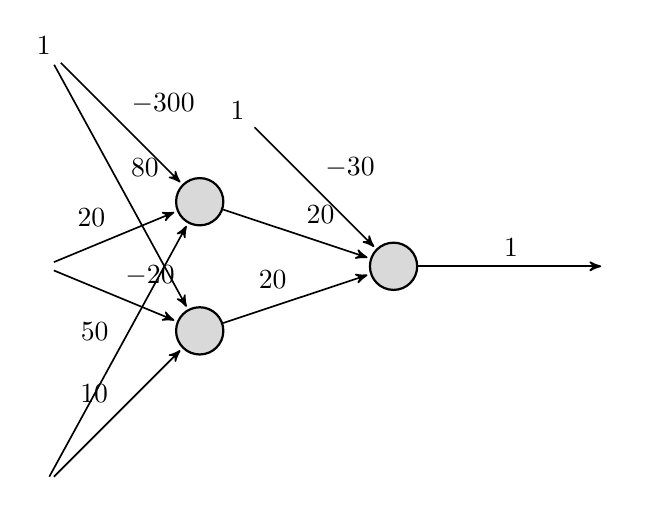
\begin{tikzpicture}[->,>=stealth',shorten >=1pt,auto,node distance=2.8cm,semithick]

  \node[input]         (A1)                    {$1$};
  \node[input]         (A2) [below of=A1] {};
  \node[input]         (A3) [below of=A2] {};
  \node[sigmoid]         (B1) [below right of=A1] {};
  \node[sigmoid]         (B2) [above right of=A3]       {};
   \node[sigmoid]         (D) [right=4cm of A2]      {};
   \node[input]         (D0)  [above left of= D]  {$1$};
 \node (E) [right of=D] {};
  \path (A1) edge node {$-300$} (B1)
            edge  node {$80$} (B2)
        (A2) edge node {$20$} (B1)
            edge  node {$-20$} (B2)
        (A3) edge node {$50$} (B1)
            edge  node {$10$} (B2)
        (B1) edge node {$20$} (D)
        (B2) edge node {$20$} (D)
        (D0) edge node {$-30$} (D)
        (D) edge node {$1$} (E);
\end{tikzpicture}

\pagebreak

\begin{tikzpicture}[->,>=stealth',shorten >=1pt,auto,node distance=2.8cm,
                    semithick]
  \tikzstyle{every state}=[fill=red,draw=none,text=white]

  \node[input]         (A1)                    {$x_0$};
  \node[input]         (A2) [below of=A1] {$x_1$};
  \node[input]         (A3) [below of=A2] {$x_2$};
   \node[sigmoid]         (D) [right of = A2 ]      {};
 \node (E) [right = 1cm of D] {$\alpha \sigma(\theta_0 x_0+\theta_1 x_1 + \theta_2x_2$)};
  \path (A1) edge node {$\theta_0$} (D)
        (A2) edge node {$\theta_1$} (D)
        (A3) edge node {$\theta_2$} (D)
        (D) edge node {$\alpha$} (E);
\end{tikzpicture}


\pagebreak

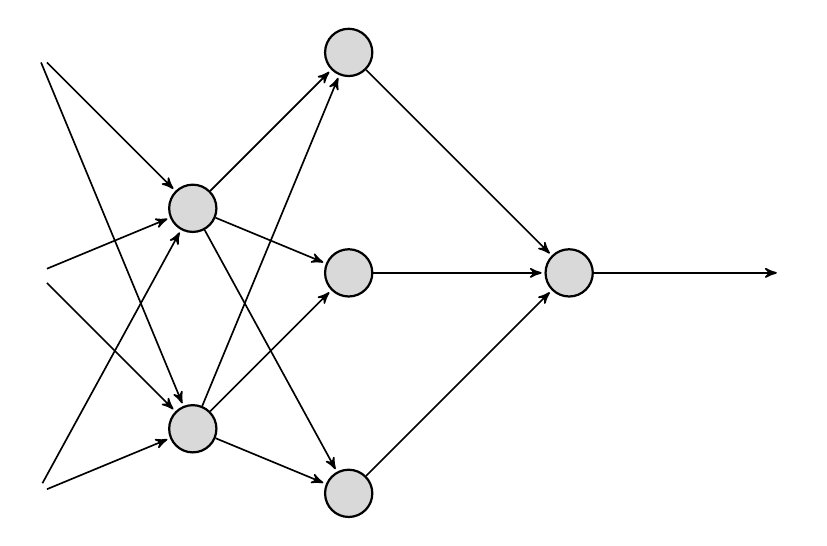
\begin{tikzpicture}[->,>=stealth',shorten >=1pt,auto,node distance=2.8cm,
                    semithick]

  \node[input]         (A1)                    {};
  \node[input]         (A2) [below of=A1] {};
  \node[input]         (A3) [below of=A2] {};
  \node[sigmoid]         (B1) [below right of=A1] {};
  \node[sigmoid]         (B2) [below of=B1]       {};
  \node[sigmoid]         (C1) [above right of=B1]            {};
  \node[sigmoid]         (C2) [below of=C1] {};
  \node[sigmoid]         (C3) [below of=C2]      {};
   \node[sigmoid]         (D) [right of=C2]      {};
 \node (E) [right of=D] {};
  \path (A1) edge node {} (B1)
            edge  node {} (B2)
        (A2) edge node {} (B1)
            edge  node {} (B2)
        (A3) edge node {} (B1)
            edge  node {} (B2)
        (B1) edge node {} (C1)
            edge  node {} (C2)
             edge  node {} (C3)
        (B2) edge node {} (C1)
            edge  node {} (C2)
             edge  node {} (C3)
        (C1) edge node {} (D)
        (C2) edge node {} (D)
        (C3) edge node {} (D)
        (D) edge node {} (E);
\end{tikzpicture}

\pagebreak

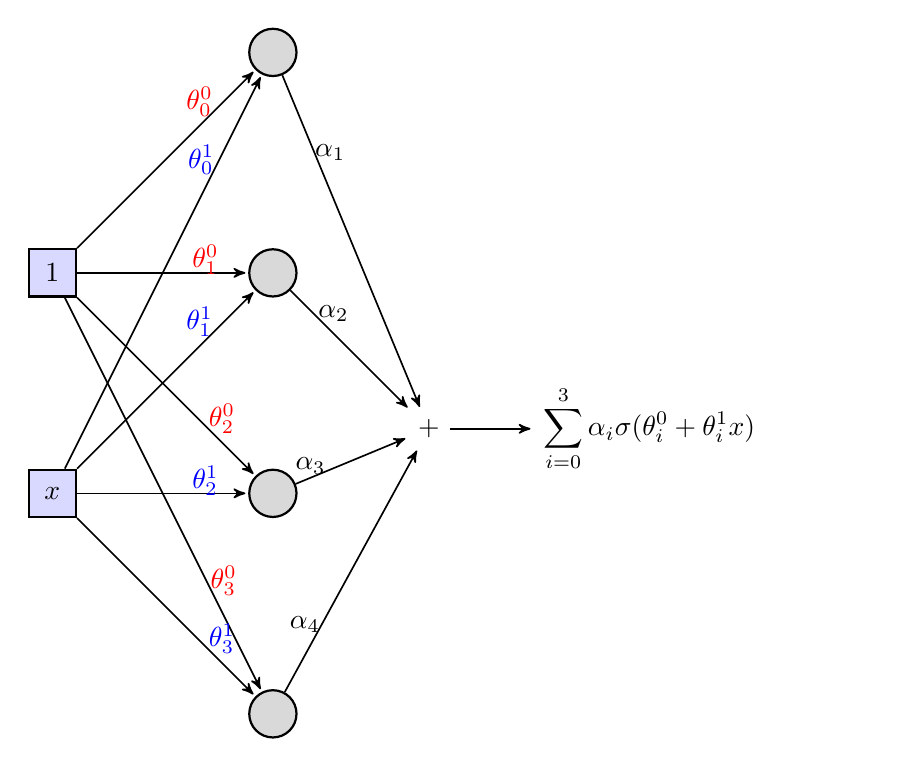
\begin{tikzpicture}[->,>=stealth',shorten >=1pt,auto,node distance=2.8cm,
                    semithick]

    \node[inputsq]  (A1) {$1$};
    \node[inputsq]  (A2) [below of=A1] {$x$};
    \node[sigmoid]  (B2) [right of=A1] {};
    \node[sigmoid]  (B1) [above of=B2] {};
    \node[sigmoid]  (B3) [below of=B2] {};
    \node[sigmoid]  (B4) [below of=B3] {};
    \node[] (C) [below right of=B2] {$+$};
    \node[] (D) [right of=C] {$\displaystyle\sum_{i=0}^3 \alpha_i \sigma(\theta^0_i+\theta^1_i x)$};
    \node (E) [right of=D] {};
    \path 
        (A1) edge node [red, near end, outer sep =-4pt] {$\theta^0_0$} (B1)
            edge  node [red, near end, outer sep =-4pt] {$\theta^0_1$} (B2)
            edge  node [red, near end, outer sep =-4pt] {$\theta^0_2$} (B3)
            edge  node [red, near end, outer sep =-4pt] {$\theta^0_3$} (B4)
        (A2) edge node [blue, near end, outer sep =-4pt] {$\theta^1_0$} (B1)
            edge  node [blue, near end, outer sep =-4pt] {$\theta^1_1$} (B2)
            edge  node [blue, near end, outer sep =-4pt] {$\theta^1_2$} (B3)
            edge  node [blue, near end, outer sep =-4pt] {$\theta^1_3$} (B4)
        (B1) edge node [near start, outer sep =-4pt]{$\alpha_1$} (C)
        (B2) edge node [near start, outer sep =-4pt] {$\alpha_2$} (C)
        (B3) edge node [near start, outer sep =-4pt] {$\alpha_3$} (C)
        (B4) edge node [near start, outer sep =-4pt] {$\alpha_4$} (C)
        (C) edge node {} (D);
\end{tikzpicture}


\end{document}
